% generated by build-figures.mjs — DO NOT EDIT
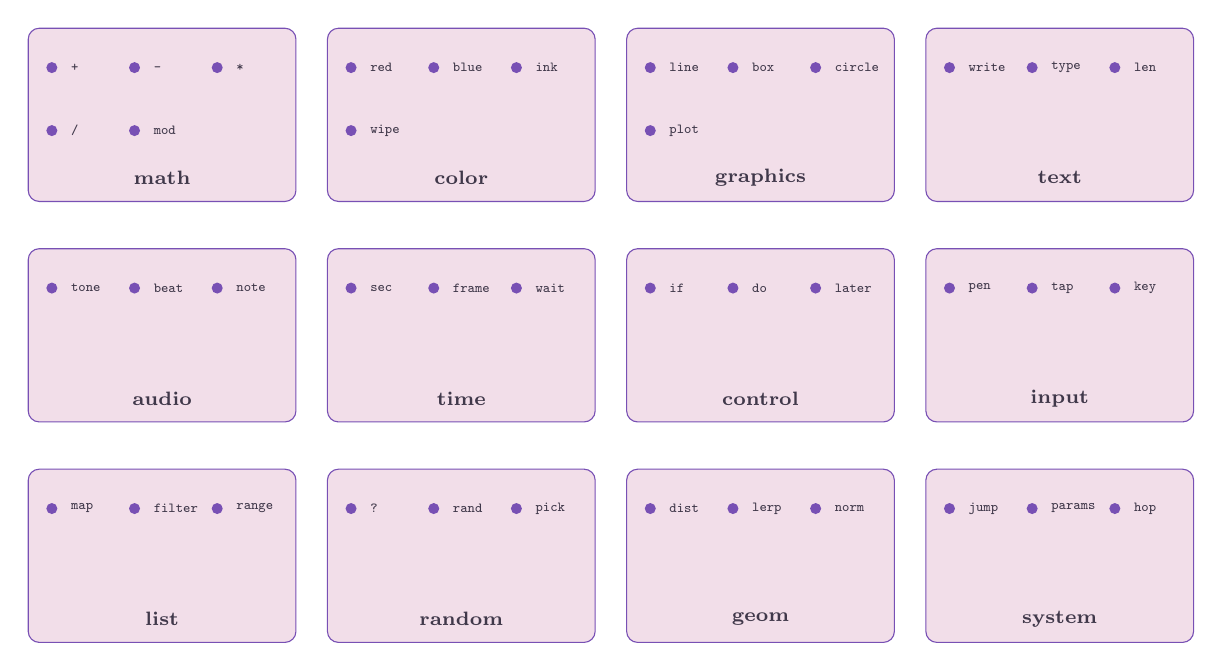
\begin{tikzpicture}[x=1mm,y=1mm]
  \definecolor{lpink}{RGB}{180,72,135}
  \definecolor{lpurple}{RGB}{120,80,180}
  \definecolor{ldark}{RGB}{64,56,74}
  \draw[lpurple,fill=lpink!18,line width=0.4pt,rounded corners=1.4mm] (4,-6) rectangle (38,-28);
  \node[font=\scriptsize\bfseries\color{ldark}] at (21,-25) {math};
  \fill[lpurple] (7,-11) circle (0.7);
  \node[font=\tiny\color{ldark},anchor=west] at (8.2,-11) {\texttt{+}};
  \fill[lpurple] (17.5,-11) circle (0.7);
  \node[font=\tiny\color{ldark},anchor=west] at (18.7,-11) {\texttt{-}};
  \fill[lpurple] (28,-11) circle (0.7);
  \node[font=\tiny\color{ldark},anchor=west] at (29.2,-11) {\texttt{*}};
  \fill[lpurple] (7,-19) circle (0.7);
  \node[font=\tiny\color{ldark},anchor=west] at (8.2,-19) {\texttt{/}};
  \fill[lpurple] (17.5,-19) circle (0.7);
  \node[font=\tiny\color{ldark},anchor=west] at (18.7,-19) {\texttt{mod}};
  \draw[lpurple,fill=lpink!18,line width=0.4pt,rounded corners=1.4mm] (42,-6) rectangle (76,-28);
  \node[font=\scriptsize\bfseries\color{ldark}] at (59,-25) {color};
  \fill[lpurple] (45,-11) circle (0.7);
  \node[font=\tiny\color{ldark},anchor=west] at (46.2,-11) {\texttt{red}};
  \fill[lpurple] (55.5,-11) circle (0.7);
  \node[font=\tiny\color{ldark},anchor=west] at (56.7,-11) {\texttt{blue}};
  \fill[lpurple] (66,-11) circle (0.7);
  \node[font=\tiny\color{ldark},anchor=west] at (67.2,-11) {\texttt{ink}};
  \fill[lpurple] (45,-19) circle (0.7);
  \node[font=\tiny\color{ldark},anchor=west] at (46.2,-19) {\texttt{wipe}};
  \draw[lpurple,fill=lpink!18,line width=0.4pt,rounded corners=1.4mm] (80,-6) rectangle (114,-28);
  \node[font=\scriptsize\bfseries\color{ldark}] at (97,-25) {graphics};
  \fill[lpurple] (83,-11) circle (0.7);
  \node[font=\tiny\color{ldark},anchor=west] at (84.2,-11) {\texttt{line}};
  \fill[lpurple] (93.5,-11) circle (0.7);
  \node[font=\tiny\color{ldark},anchor=west] at (94.7,-11) {\texttt{box}};
  \fill[lpurple] (104,-11) circle (0.7);
  \node[font=\tiny\color{ldark},anchor=west] at (105.2,-11) {\texttt{circle}};
  \fill[lpurple] (83,-19) circle (0.7);
  \node[font=\tiny\color{ldark},anchor=west] at (84.2,-19) {\texttt{plot}};
  \draw[lpurple,fill=lpink!18,line width=0.4pt,rounded corners=1.4mm] (118,-6) rectangle (152,-28);
  \node[font=\scriptsize\bfseries\color{ldark}] at (135,-25) {text};
  \fill[lpurple] (121,-11) circle (0.7);
  \node[font=\tiny\color{ldark},anchor=west] at (122.2,-11) {\texttt{write}};
  \fill[lpurple] (131.5,-11) circle (0.7);
  \node[font=\tiny\color{ldark},anchor=west] at (132.7,-11) {\texttt{type}};
  \fill[lpurple] (142,-11) circle (0.7);
  \node[font=\tiny\color{ldark},anchor=west] at (143.2,-11) {\texttt{len}};
  \draw[lpurple,fill=lpink!18,line width=0.4pt,rounded corners=1.4mm] (4,-34) rectangle (38,-56);
  \node[font=\scriptsize\bfseries\color{ldark}] at (21,-53) {audio};
  \fill[lpurple] (7,-39) circle (0.7);
  \node[font=\tiny\color{ldark},anchor=west] at (8.2,-39) {\texttt{tone}};
  \fill[lpurple] (17.5,-39) circle (0.7);
  \node[font=\tiny\color{ldark},anchor=west] at (18.7,-39) {\texttt{beat}};
  \fill[lpurple] (28,-39) circle (0.7);
  \node[font=\tiny\color{ldark},anchor=west] at (29.2,-39) {\texttt{note}};
  \draw[lpurple,fill=lpink!18,line width=0.4pt,rounded corners=1.4mm] (42,-34) rectangle (76,-56);
  \node[font=\scriptsize\bfseries\color{ldark}] at (59,-53) {time};
  \fill[lpurple] (45,-39) circle (0.7);
  \node[font=\tiny\color{ldark},anchor=west] at (46.2,-39) {\texttt{sec}};
  \fill[lpurple] (55.5,-39) circle (0.7);
  \node[font=\tiny\color{ldark},anchor=west] at (56.7,-39) {\texttt{frame}};
  \fill[lpurple] (66,-39) circle (0.7);
  \node[font=\tiny\color{ldark},anchor=west] at (67.2,-39) {\texttt{wait}};
  \draw[lpurple,fill=lpink!18,line width=0.4pt,rounded corners=1.4mm] (80,-34) rectangle (114,-56);
  \node[font=\scriptsize\bfseries\color{ldark}] at (97,-53) {control};
  \fill[lpurple] (83,-39) circle (0.7);
  \node[font=\tiny\color{ldark},anchor=west] at (84.2,-39) {\texttt{if}};
  \fill[lpurple] (93.5,-39) circle (0.7);
  \node[font=\tiny\color{ldark},anchor=west] at (94.7,-39) {\texttt{do}};
  \fill[lpurple] (104,-39) circle (0.7);
  \node[font=\tiny\color{ldark},anchor=west] at (105.2,-39) {\texttt{later}};
  \draw[lpurple,fill=lpink!18,line width=0.4pt,rounded corners=1.4mm] (118,-34) rectangle (152,-56);
  \node[font=\scriptsize\bfseries\color{ldark}] at (135,-53) {input};
  \fill[lpurple] (121,-39) circle (0.7);
  \node[font=\tiny\color{ldark},anchor=west] at (122.2,-39) {\texttt{pen}};
  \fill[lpurple] (131.5,-39) circle (0.7);
  \node[font=\tiny\color{ldark},anchor=west] at (132.7,-39) {\texttt{tap}};
  \fill[lpurple] (142,-39) circle (0.7);
  \node[font=\tiny\color{ldark},anchor=west] at (143.2,-39) {\texttt{key}};
  \draw[lpurple,fill=lpink!18,line width=0.4pt,rounded corners=1.4mm] (4,-62) rectangle (38,-84);
  \node[font=\scriptsize\bfseries\color{ldark}] at (21,-81) {list};
  \fill[lpurple] (7,-67) circle (0.7);
  \node[font=\tiny\color{ldark},anchor=west] at (8.2,-67) {\texttt{map}};
  \fill[lpurple] (17.5,-67) circle (0.7);
  \node[font=\tiny\color{ldark},anchor=west] at (18.7,-67) {\texttt{filter}};
  \fill[lpurple] (28,-67) circle (0.7);
  \node[font=\tiny\color{ldark},anchor=west] at (29.2,-67) {\texttt{range}};
  \draw[lpurple,fill=lpink!18,line width=0.4pt,rounded corners=1.4mm] (42,-62) rectangle (76,-84);
  \node[font=\scriptsize\bfseries\color{ldark}] at (59,-81) {random};
  \fill[lpurple] (45,-67) circle (0.7);
  \node[font=\tiny\color{ldark},anchor=west] at (46.2,-67) {\texttt{?}};
  \fill[lpurple] (55.5,-67) circle (0.7);
  \node[font=\tiny\color{ldark},anchor=west] at (56.7,-67) {\texttt{rand}};
  \fill[lpurple] (66,-67) circle (0.7);
  \node[font=\tiny\color{ldark},anchor=west] at (67.2,-67) {\texttt{pick}};
  \draw[lpurple,fill=lpink!18,line width=0.4pt,rounded corners=1.4mm] (80,-62) rectangle (114,-84);
  \node[font=\scriptsize\bfseries\color{ldark}] at (97,-81) {geom};
  \fill[lpurple] (83,-67) circle (0.7);
  \node[font=\tiny\color{ldark},anchor=west] at (84.2,-67) {\texttt{dist}};
  \fill[lpurple] (93.5,-67) circle (0.7);
  \node[font=\tiny\color{ldark},anchor=west] at (94.7,-67) {\texttt{lerp}};
  \fill[lpurple] (104,-67) circle (0.7);
  \node[font=\tiny\color{ldark},anchor=west] at (105.2,-67) {\texttt{norm}};
  \draw[lpurple,fill=lpink!18,line width=0.4pt,rounded corners=1.4mm] (118,-62) rectangle (152,-84);
  \node[font=\scriptsize\bfseries\color{ldark}] at (135,-81) {system};
  \fill[lpurple] (121,-67) circle (0.7);
  \node[font=\tiny\color{ldark},anchor=west] at (122.2,-67) {\texttt{jump}};
  \fill[lpurple] (131.5,-67) circle (0.7);
  \node[font=\tiny\color{ldark},anchor=west] at (132.7,-67) {\texttt{params}};
  \fill[lpurple] (142,-67) circle (0.7);
  \node[font=\tiny\color{ldark},anchor=west] at (143.2,-67) {\texttt{hop}};
\end{tikzpicture}
